%
% Iniciando o documento
%
\documentclass[spectratio=43, portuguese]{beamer}
\usepackage[utf8]{inputenc}
\usepackage[brazil]{babel}
\usepackage[alf]{abntex2cite}	% Citações padrão ABNT
\usepackage{tikz}
\usepackage{graphicx}			% Inclusão de gráficos
\usepackage[T1]{fontenc}		% Selecao de codigos de fonte
%\usepackage[utf8x]{inputenc}	% Codificacao do documento (conversão automática dos acentos)
\usepackage{longtable}
\usepackage{smartdiagram}
\usepackage{enumerate}
\usepackage{subcaption}
\setlength{\LTpost}{0pt}
\setlength{\LTpre}{0pt}
\usepackage{pgfplots}
\pgfplotsset{compat=1.8}
\setbeamertemplate{caption}[numbered]
% O comando abaixo desabilita a barra de navegação
\setbeamertemplate{navigation symbols}{}
%
% Escolhendo o tema e seu esquema de cores
% Facilitador: https://hartwork.org/beamer-theme-matrix/
%
\usetheme{Darmstadt}
\usecolortheme{crane}
%
% Inicia - Definir o slide mestre
%
\title{Implantação de ligação ferroviária ao longo do curso do rio Tietê na Região Metropolitana de São Paulo}
\subtitle{Comparação com a infraestrutura existente ao longo do curso do rio Pinheiros}
\author{
	Caio César Carvalho Ortega\\
	}
\date{\today}
%
% Inserindo um logotipo
% 
\titlegraphic{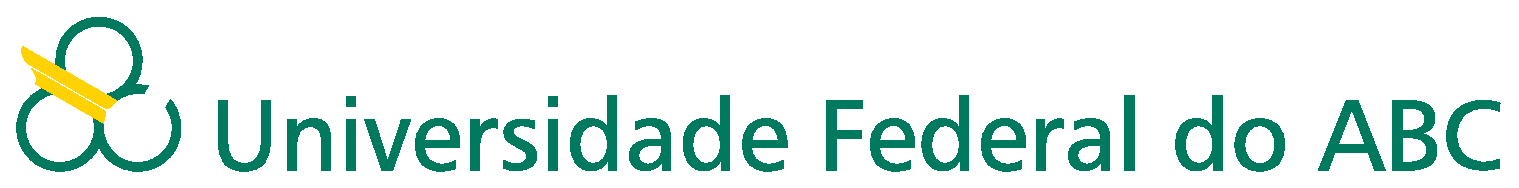
\includegraphics[width=10.0cm]{img/logotipo-ufabc-extenso.eps}\hspace*{0cm}
\logo{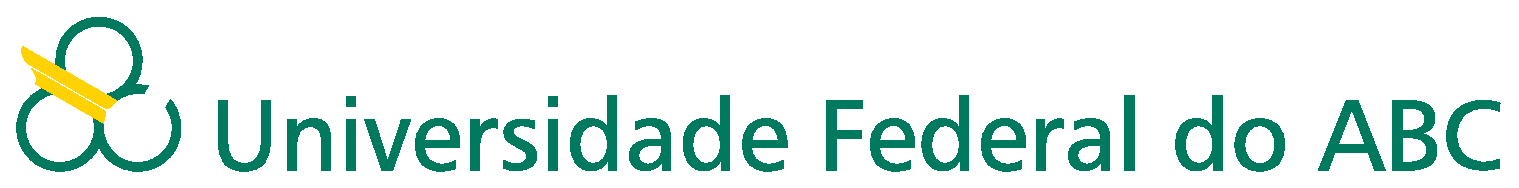
\includegraphics[height=0cm]{img/logotipo-ufabc-extenso.eps}}
}
%
% Conclui - Definir o slide mestre 
%
\begin{document}
\begin{frame}
\titlepage
\end{frame}
%
% A apresentação "de facto" começa a partir daqui
%
% ---
% Orientações:
% Cada apresentação deve durar 10 minutos, seguida de 3 minutos de perguntas. Apresente claramente sua pergunta, hipótese e principais pontos da argumentação; fique à vontade para projetar imagens ou citações (suas ou de outros autores).
% ---
%
% ----------------- NOVA SEÇÃO --------------------------------

\section{Pergunta e hipótese}

% ----------------- NOVO SLIDE --------------------------------

\begin{frame}{Motivação}
	
	\begin{itemize}
		\item Assimetria entre a infraestrutura de transporte existente ao longo do curso dos rios Pinheiros e Tietê na RMSP
		\item Processos de urbanização e alteração do meio físico distintos entre os dois rios
		\begin{itemize}
			\item Pinheiros: retificado pela Light
			\item Tietê: retificado pelo poder público
		\end{itemize}
		\item Inserção dos dois cursos d'água ``no contexto urbano das últimas quatro décadas, sendo a construção das avenidas marginais, aliada às obras de retificação e canalização, a consolidação dessa atitude'' \cite[p. 43]{monteiro2010a}
		\item Considerar especialmente a caráter estratégico das várzeas \cite[p. 63]{franco2005a} e o ``o papel das ferrovias ao conectar pontos distantes do espaço ocupado pela metrópole'' \cite[p. 63]{franco2005a}
	\end{itemize}
	
\end{frame}

% ----------------- NOVO SLIDE --------------------------------

\begin{frame}{Pergunta}
	
	\begin{block}
		{\large Considerando que há uma ligação ferroviária que acompanha o curso do rio Pinheiros, faria sentido implantar outra acompanhando o curso do rio Tietê em, pelo menos, parte da Região Metropolitana de São Paulo?}
	\end{block}
	
	\begin{figure}
		\centering
		\caption{Marginal Tietê em 2013, observada a partir da Linha 7-Rubi da CPTM}
		\label{fig:mtiete_l7}
		\includegraphics[width=0.8\linewidth]{img/13020087}
		\subcaption*{Fonte: elaboração própria}
	\end{figure}
	
\end{frame}

% ----------------- NOVO SLIDE --------------------------------

\begin{frame}{Hipótese}
	
	A hipótese é de que a implantação seria positiva, para tanto, são considerados como fatores:
	
	\begin{itemize}
		\item Viagens realizadas pela Marginal Tietê
		\item Possibilidade de aproximar a população do rio e a configuração formada pela Marginal Tietê paralela (ainda que em parte) às linhas 3-Vermelha (esta da CMSP), 11-Coral, 12-Safira, 7-Rubi e 8-Diamante (estas últimas da CPTM)
		\item Densidade de estações por km$^{2}$
		\item Densidade de conexões entre linhas que se cruzam por km$^{2}$
		\item Ganho de capacidade/hora
	\end{itemize}
	
\end{frame}

% ----------------- NOVO SLIDE --------------------------------

\begin{frame}{Observações adicionais}

	\begin{alertblock}{Cabe ainda salientar que\dots}
		\dots {\huge a implantação de uma nova linha do sistema metroferroviário não é aqui pensada como uma obra de engenharia, mas como uma decisão política e de planejamento territorial}
	\end{alertblock}
	
	Pretende-se: (i) resgatar o contexto histórico; (ii) realizar uma breve comparação dos processos de urbanização e; (iii) refletir objetivamente acerca do possível impacto

\end{frame}

% ----------------- NOVA SEÇÃO --------------------------------

\section{Argumentação}

% ----------------- NOVO SLIDE --------------------------------

\begin{frame}{Delimitação da área de estudo}
	
	Fatores hidrográficos que contribuíram para que eu me voltasse a uma parcela da Região Metropolitana de São Paulo:
	
	\begin{itemize}
		\item Bacia sedimentar: ``situada no interior do planalto Atlântico, a região metropolitana está implantada na bacia sedimentar de São Paulo, por entre a Serra do Mar (ao sul) e da Cantareira (ao norte)'' \cite[p. 35]{monteiro2010a}
		\item Várzea do rio Tietê: ``a várzea do rio Tietê estende-se em 25 km do bairro da Penha a Osasco, numa largura que varia entre 1,5 a 2,5km. Já a várzea do Pinheiros, de Santo Amaro até o Tietê, estende-se em 20 km, numa largura entre 1 a 1,5km'' \cite[p. 35]{monteiro2010a}
	\end{itemize}
	
\end{frame}

% ----------------- NOVO SLIDE --------------------------------

\begin{frame}{Espaço para algum ineditismo}
	
	Estudos atuais contribuem para ampliar a compreensão do território ligado ao rio Tietê e diferenciar sua retificação em relação àquela realizada no Pinheiros, ligada aos negócios da Cia. City \cite[p. 53]{francca2000a}. Estes, entretanto, não respondem à pergunta colocada por mim. Não encontrei teses ou artigos que \textbf{se debrucem especificamente sobre a possibilidade de construir uma ferrovia metropolitana ao longo do Tietê}.
	
	\begin{figure}
		\centering
		\caption{Dormente com a marca da Fepasa na Estação Cidade Jardim da CPTM em 2013}
		\label{fig:dormente_fepasa}
		\includegraphics[width=0.5\linewidth]{img/DSCN2006}
		\subcaption*{Fonte: elaboração própria}
	\end{figure}
	
\end{frame}

% ----------------- NOVO SLIDE --------------------------------

\begin{frame}{Questão do acesso à cidade}
	
	\begin{columns}
		
		\column{0.6\textwidth}
		Conveniência sem distinção de renda, como \citeonline[p. 149]{requena2016a} salienta com relação à Linha 9-Esmeralda: ``sua conveniência reside no fato de proporcionar, principalmente ao cidadão de menor renda, meios eficazes de acessar as áreas mais equipadas da cidade para seu uso, independentemente de suas condições financeiras'', trata-se de um atributo inexistente ao longo da Marginal Tietê, na qual o transporte individual motorizado é o principal protagonista como forma de acesso, conforme reflexão feita por \citeonline[p. 147--149]{franco2005a}
		
		\column{0.4\textwidth}
		\begin{figure}
			\centering
			\caption{Plataforma sentido Grajaú da Estação Pinheiros, 2018}
			\label{fig:plat_pin}
			\includegraphics[width=0.65\linewidth]{img/IMG_5838}
			\subcaption*{Fonte: elaboração própria}
		\end{figure}
	\end{columns}
	
\end{frame}

% ----------------- NOVO SLIDE --------------------------------

\begin{frame}{Questão da paisagem}
	
A seguinte constatação de \citeonline[p. 148--149]{monteiro2010a} também foi suficientemente intrigante para que eu desse continuidade a este projeto:

\begin{quote}
	``Curiosamente, portanto, ainda que se interponha entre o rio e a cidade como mais um elemento de obstáculo ao acesso direto aos rios, a via férrea da CPTM acaba por levar a população às margens dos rios duma outra maneira, ainda que não seja o Pinheiros o lugar de destino intencionado. As estações de trem, nesse sentido, compostas por um edifício de acesso na malha urbana, uma passarela sobre a via expressa e a plataforma, convertem-se em importantes elementos de acesso às mensagens contidas no sistema marginal''.
\end{quote}

\end{frame}

% ----------------- NOVO SLIDE --------------------------------

\begin{frame}{E a própria paisagem}

	\begin{figure}
		\centering
		\caption{Estação Socorro observada a partir do mezanino da Estação Santo Amaro, 2013}
		\label{fig:trilhos_cjd}
		\includegraphics[width=0.65\linewidth]{img/DSCN2032}
		\subcaption*{Fonte: elaboração própria}
	\end{figure}
	
\end{frame}

% ----------------- NOVO SLIDE --------------------------------

\begin{frame}{Metodologia}
	
	\begin{itemize}
		\item Realização de uma pesquisa exploratória, envolvendo revisão bibliográfica pelo menos das obras contidas no projeto, sendo uma delas parte dos trabalhos desenvolvidos pelo grupo Metrópole Fluvial da FAU-USP
		\item Serão utilizados dados da Prefeitura do Município de São Paulo, especialmente da CET, além disso, prevê-se a utilização de dados do Governo do Estado de São Paulo, especialmente aqueles ligados à demanda e volume de passageiros da CMSP e da CPTM
		\item Para a elaboração de representações cartográficas das áreas de estudo, prevejo a utilização de \textit{shapefiles} do IBGE, da Emplasa e da SMUL da PMSP, a serem utilizados em conjunto com o \textit{software} de SIG QGIS.
	\end{itemize}
	
\end{frame}

% ----------------- NOVA SEÇÃO --------------------------------

\section{Referências}

% ----------------- NOVO SLIDE --------------------------------

% --- O comando \allowframebreaks ---
% Se o conteúdo não se encaixa em um quadro, a opção allowframebreaks instrui 
% beamer para quebrá-lo automaticamente entre dois ou mais quadros,
% mantendo o frametitle do primeiro quadro (dado como argumento) e acrescentando 
% um número romano ou algo parecido na continuação.

\begin{frame}[allowframebreaks]{Referências}
	\bibliography{fontes}
\end{frame}

% ----------------- FIM DO DOCUMENTO -----------------------------------------
\end{document}